\section{Detector Model}
\label{sec:detector_description}

In order to study the topology of $\vbb$ decay and background events in a liquid scintillator detector, a Geant4\cite{geant4one,geant4two} simulation has been constructed. This is the same simulation used in our preceding paper~\cite{Aberle2014}. Therefore, we limit out discussion of the simulation to a summary of the the most relevant simulation parameters.

The simulation uses Geant4~version 4.9.6.  We use the default liquid scintillator optical model, in which optical photons are assigned the group velocity in the wavelength region of normal dispersion.

The detector geometry is a sphere of 6.5~m radius filled with
scintillator. The default scintillator composition has been chosen to match a KamLAND-like
scintillator\cite{kamland2003}: 80\% n-dodecane, 20\% pseudocumene and 1.52~g/l PPO. The
scintillator properties implemented in the simulation include 
\begin{itemize}
\item the atomic composition and density ($\rho$ = 0.78~g/ml), 
\item the wavelength-dependent attenuation length\cite{tajimaMaster} and refractive index\cite{OlegThesis}, 
\item the scintillation emission spectrum\cite{tajimaMaster}, 
\item emission rise time ($\tau_r$ = 1.0~ns) and emission decay time constants ($\tau_{d1}$ = 6.9~ns and $\tau_{d2}$ = 8.8~ns with relative weights of 0.87 and 0.13)\cite{tajimaThesis}, 
\item scintillator light yield (9030 photons/MeV), and 
\item the Birks constant ($kB$ $\approx$ 0.1~mm/MeV)\cite{ChrisThesis}.  
\end{itemize}
The attenuation length at 400~nm, which is the position of the peak standard bialkali photocathode efficiency, is 25~m. The attenuation length drops precipitously from 6.5~m to 0.65~m between 370~nm and 360~nm. We use this drop to define the cutoff wavelength at 370~nm. This is a standard scintillator. However, we do deviate from the baseline KamLAND case in that the re-emission of absorbed photons in the scintillator bulk volume and optical scattering, specifically Rayleigh scattering, has not yet been included. A test simulation shows that the effect of optical scattering is negligible~\cite{Aberle2014}.

The inner sphere surface is used as the photodetector. It is treated
as fully absorbing (no reflections), with a photodetector coverage of
100\%. As in the case of optical scattering, reflections at the sphere are a small effect that would create a small tail at longer times. The default is the QE of a bialkali photocathode (Hamamatsu
R7081 PMT)\cite{Hamamatsu_R7081}. The QE values as a function of wavelength come from the Double Chooz\cite{dctwo}
Monte Carlo simulation. We note that the KamLAND 17-inch PMTs use the
same photocathode type with similar quantum efficiency. We are neglecting any threshold effects in the photodetector readout electronics.


Four effects primarily contribute to the timing of the scintillator detector
system: the travel time of the particle, the time constants of the scintillation process, chromatic dispersion, and the timing of the photodetector.

In the energy range important for $0\nu\beta\beta$, a 1.4~MeV electron travels a total path length of 0.8~cm, has a distance from the origin of 0.6~cm in 0.030$\pm$0.004~ns  and takes 0.028$\pm$0.004~ns to drop below Cherenkov threshold. We note that due to scattering of the electron, the final direction of the electron before it stops does not correspond to the initial direction; however the scattering angle is small while the majority of Cherenkov light is produced. The Cherenkov light thus still encodes the direction of the primary electron. The scattering physics is handled by Geant4's ``Multiple Scattering" process which is valid down to 1~keV, where atomic shell structure becomes important\cite{geant4scatt}.


The scintillator-specific rise and decay times are the second effect that determines the timing in a scintillator detector. The first step in the scintillation process is the transfer of energy from the solvent to the solute. The time constant of this
energy transfer accounts for a rise time in scintillation light
emission. Because past neutrino experiments were not highly sensitive to the
effect of the scintillation rise time, there is a lack of accurate measurements of this property. We assume a rise time of 1.0~ns -- but more
detailed studies are needed in the future. The two time constants used
to describe the falling edge of the scintillator emission time
distribution (quoted above) are values specific to the KamLAND scintillator.

Chromatic dispersion is the third effect that determines the timing in a scintillator detector. Due to the wavelength-dependence of the refractive index the speed of
light in the scintillator increases
with increasing photon wavelengths for normal dispersion, with red
light traveling faster than blue light.

Photoelectrons coming from Cherenkov light are on average
created about 0.5~ns earlier than PEs from scintillation light. The
RMS values from PE time distributions for Cherenkov and scintillation
light are both about 0.5~ns. Note that these numbers include the
effect of the finite electron travel time.

The fourth effect determining the timing in a scintillator detector is the timing of the photodetectors. The measurement of the arrival times of single photoelectrons is
affected by the transit-time spread (TTS) of the photodetectors, a
number which can be different by orders of magnitude depending on the
detector type. We use a TTS of 0.1~ns ($\sigma$), which can be achieved with large area picosecond photodetectors
(LAPPDs)\cite{Adams:2013nva,RSI_paper,PSEC4_paper,anode_paper} and possibly hybrid photodetectors
(HPDs)\cite{hpdThesis}; even significantly lower TTS numbers are
realistic with the LAPPD\cite{RSI_paper,PSEC4_paper,anode_paper}.

The primary quantities provided by the Geant4~simulation are the photoelectron hit
positions and the detection times after the TTS resolution has been
applied. These quantities are then used for event topology reconstruction.

Figures~\ref{fig:ArrivalTimeDist} and~\ref{fig:NPhotDist} show the output of the detector simulation discussed in this section. Left panel in Fig.~\ref{fig:ArrivalTimeDist} compares PE arrival time between Cherenkov and scintillation light for 1000 simulated $\Te$ $\vbb$-decay events. The right panel in Fig.~\ref{fig:ArrivalTimeDist} compares the Cherenkov PE arrival times between $\Te$ $\vbb$-decay and $\B$ events. $\B$ events produce a slightly higher number of the Cherenkov photons because they have only one electron carrying the same kinetic energy as opposed to the two electrons in the case of $\vbb$-decay events. Distributions of the scintillation PEs' arrival time are indistinguishable between $^{130}$Te 0{\nbb} decay and $^8$B due to identical total energy in the event, $Q(^{130}{\rm Te})=2.526$~MeV.

\begin{figure*}[ht]
  \centering
  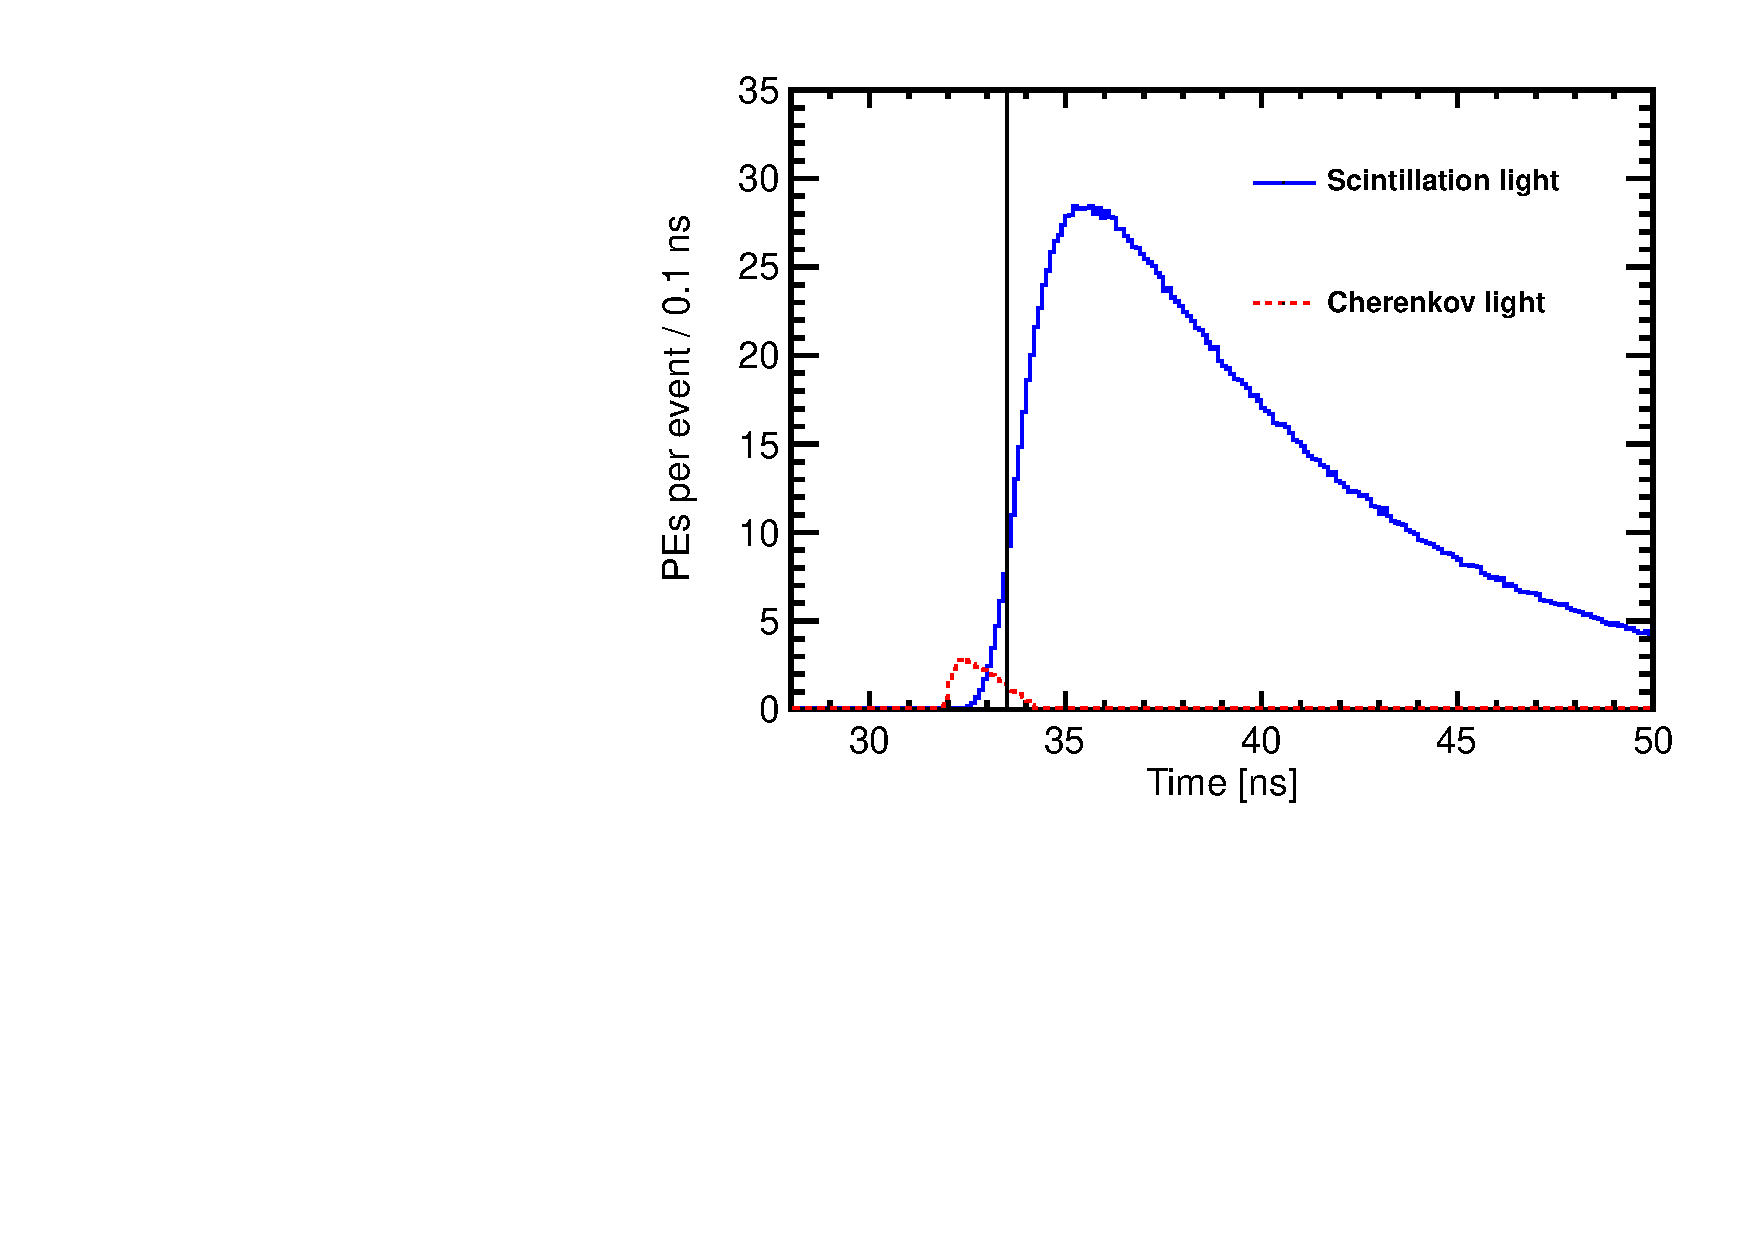
\includegraphics[width=0.45\textwidth]{hT_Te130.pdf}
  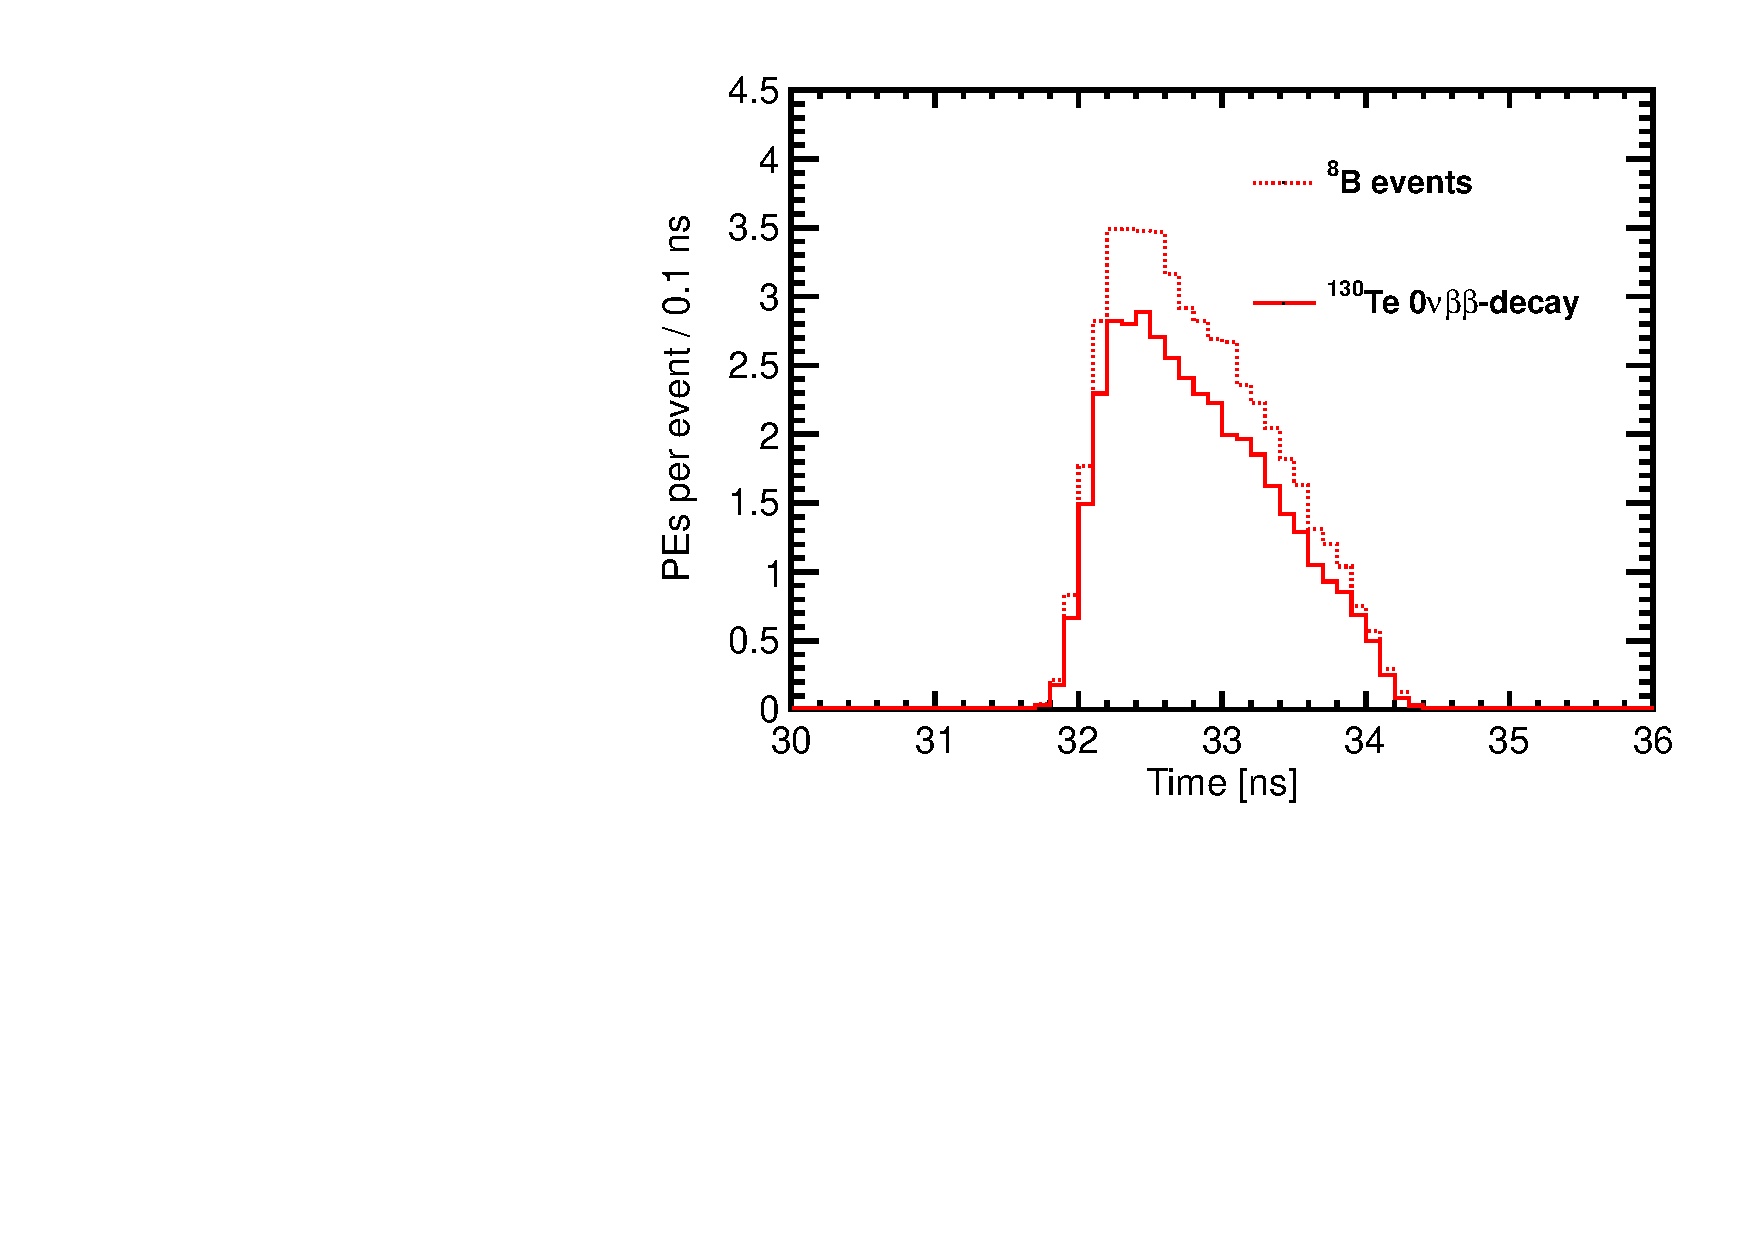
\includegraphics[width=0.45\textwidth]{hTche_Te130_B8.pdf}
  \caption{\emph{Left:} Photo-electron (PE) arrival times after
    application of the photo-detector transit time spread (TTS) of
    100~ps for the simulation of 1000 0{\nbb} decay events of
    $^{130}$Te at the center of the detector. PEs from Cherenkov light
    (\emph{dashed red line}) and scintillation light (\emph{solid blue
      line}) are compared. The black vertical line illustrates a time
    cut at 33.5 ns. \emph{Right:} Comparison between Cherenkov PEs
    arrival time for $^{130}$Te {0\nbb} decay (\emph{solid line}) and
    $^{8}$B (\emph{dotted line}) events. {\bf Distributions of the
      scintillation PEs arrival time are indistinguishable between
      $^{130}$Te 0{\nbb} decay and $^8$B due to identical total energy
      in the event, $Q(^{130}{\rm Te})=2.526$~MeV.} }
\label{fig:ArrivalTimeDist}
\end{figure*}

As shown in Fig.~\ref{fig:ArrivalTimeDist}, a time cut of 33.5~ns on the PE arrival time selects a sample of early PEs that includes the majority of Cherenkov photons. Scintillation PEs also are selected with this time cut. Figure~\ref{fig:NPhotDist} shows the total number of scintillation and Cherenkov PE per event for $\vbb$ signal and $\B$ background events. 
The higher number of Cherenkov PE produces in single electron event topology early PE sample has on average slightly higher number of PE. This difference is not significant enough to be used alone as a reliable discriminant between $\vbb$-decay and $\B$ events. However it may provide an extra handle on signal-background separation in combination (e.g. by using multivariative techniques) with other event parameters.

\begin{figure*}[ht]
  \centering
  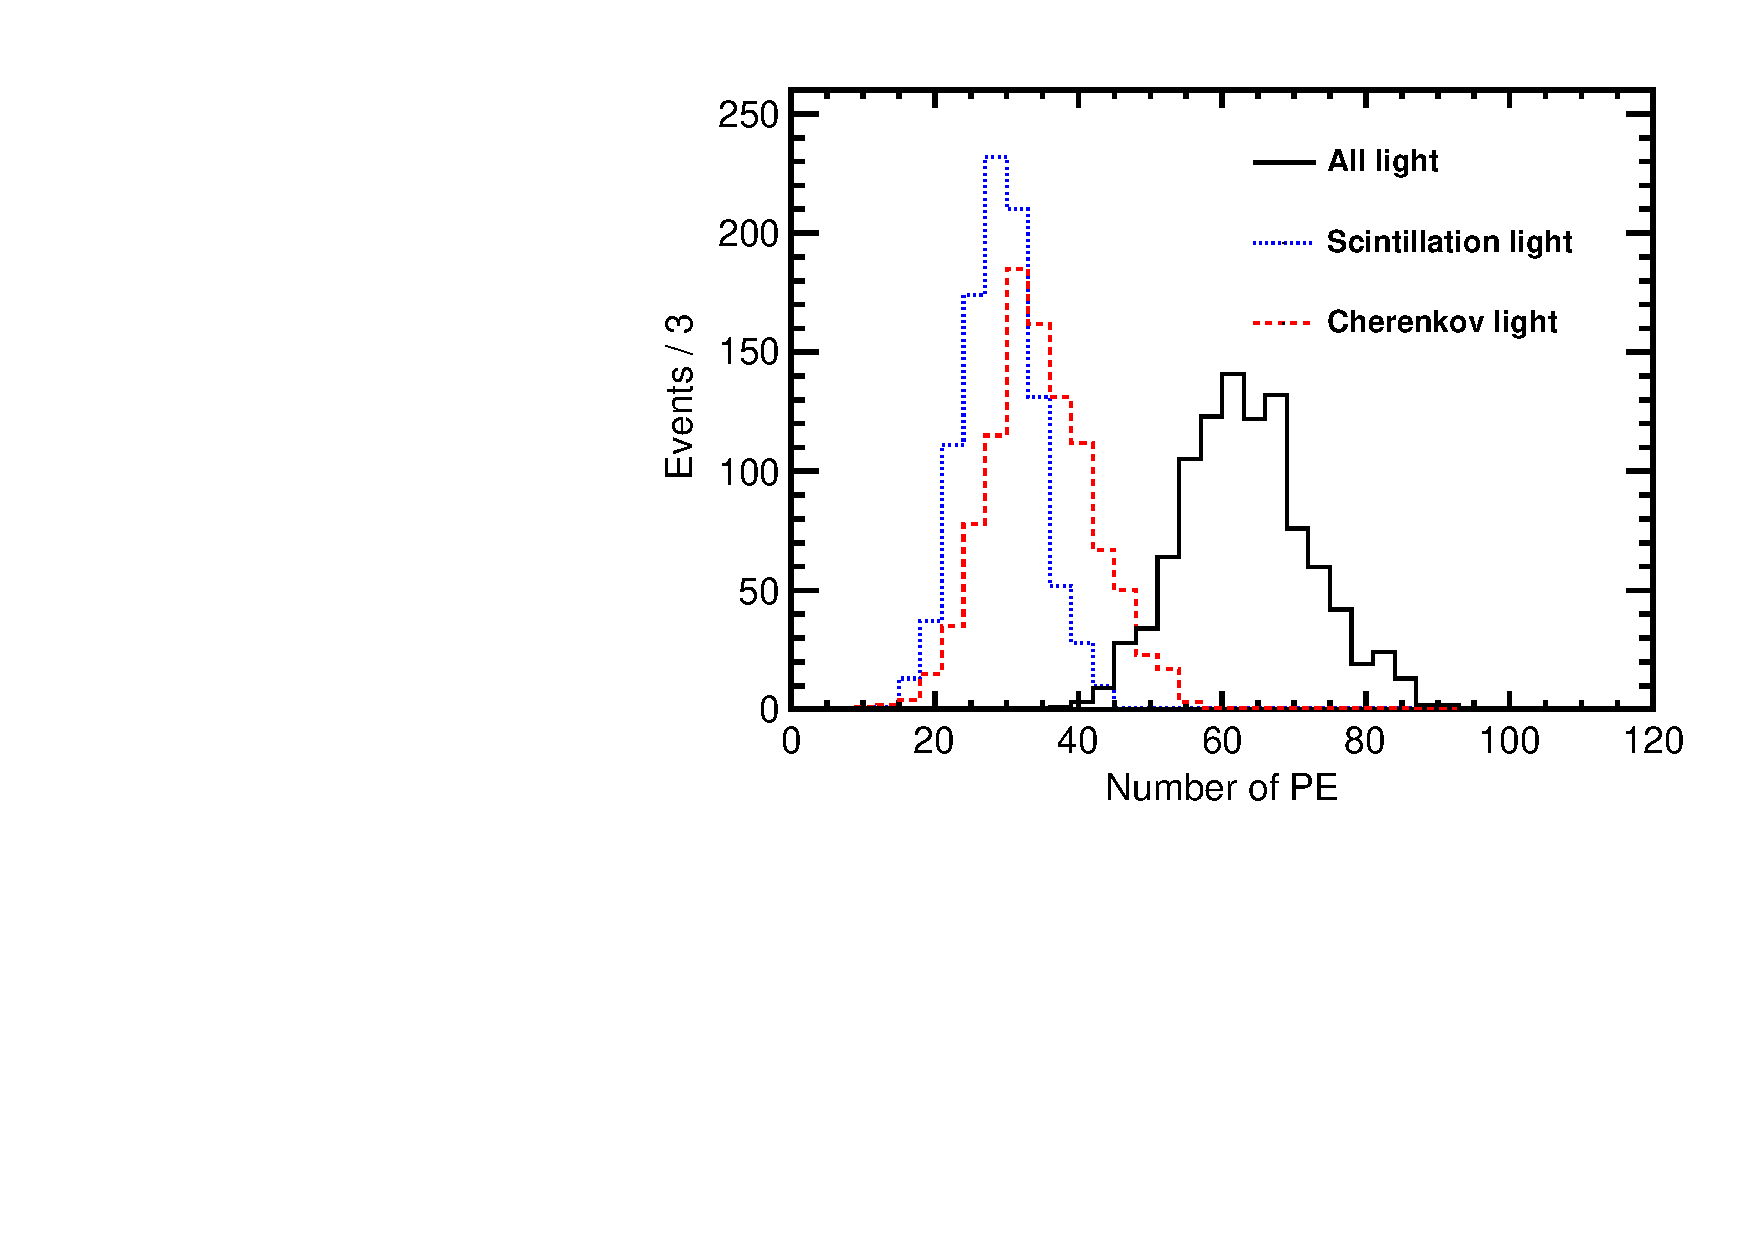
\includegraphics[width=0.45\textwidth]{hMomNPhot_Te130.pdf}
  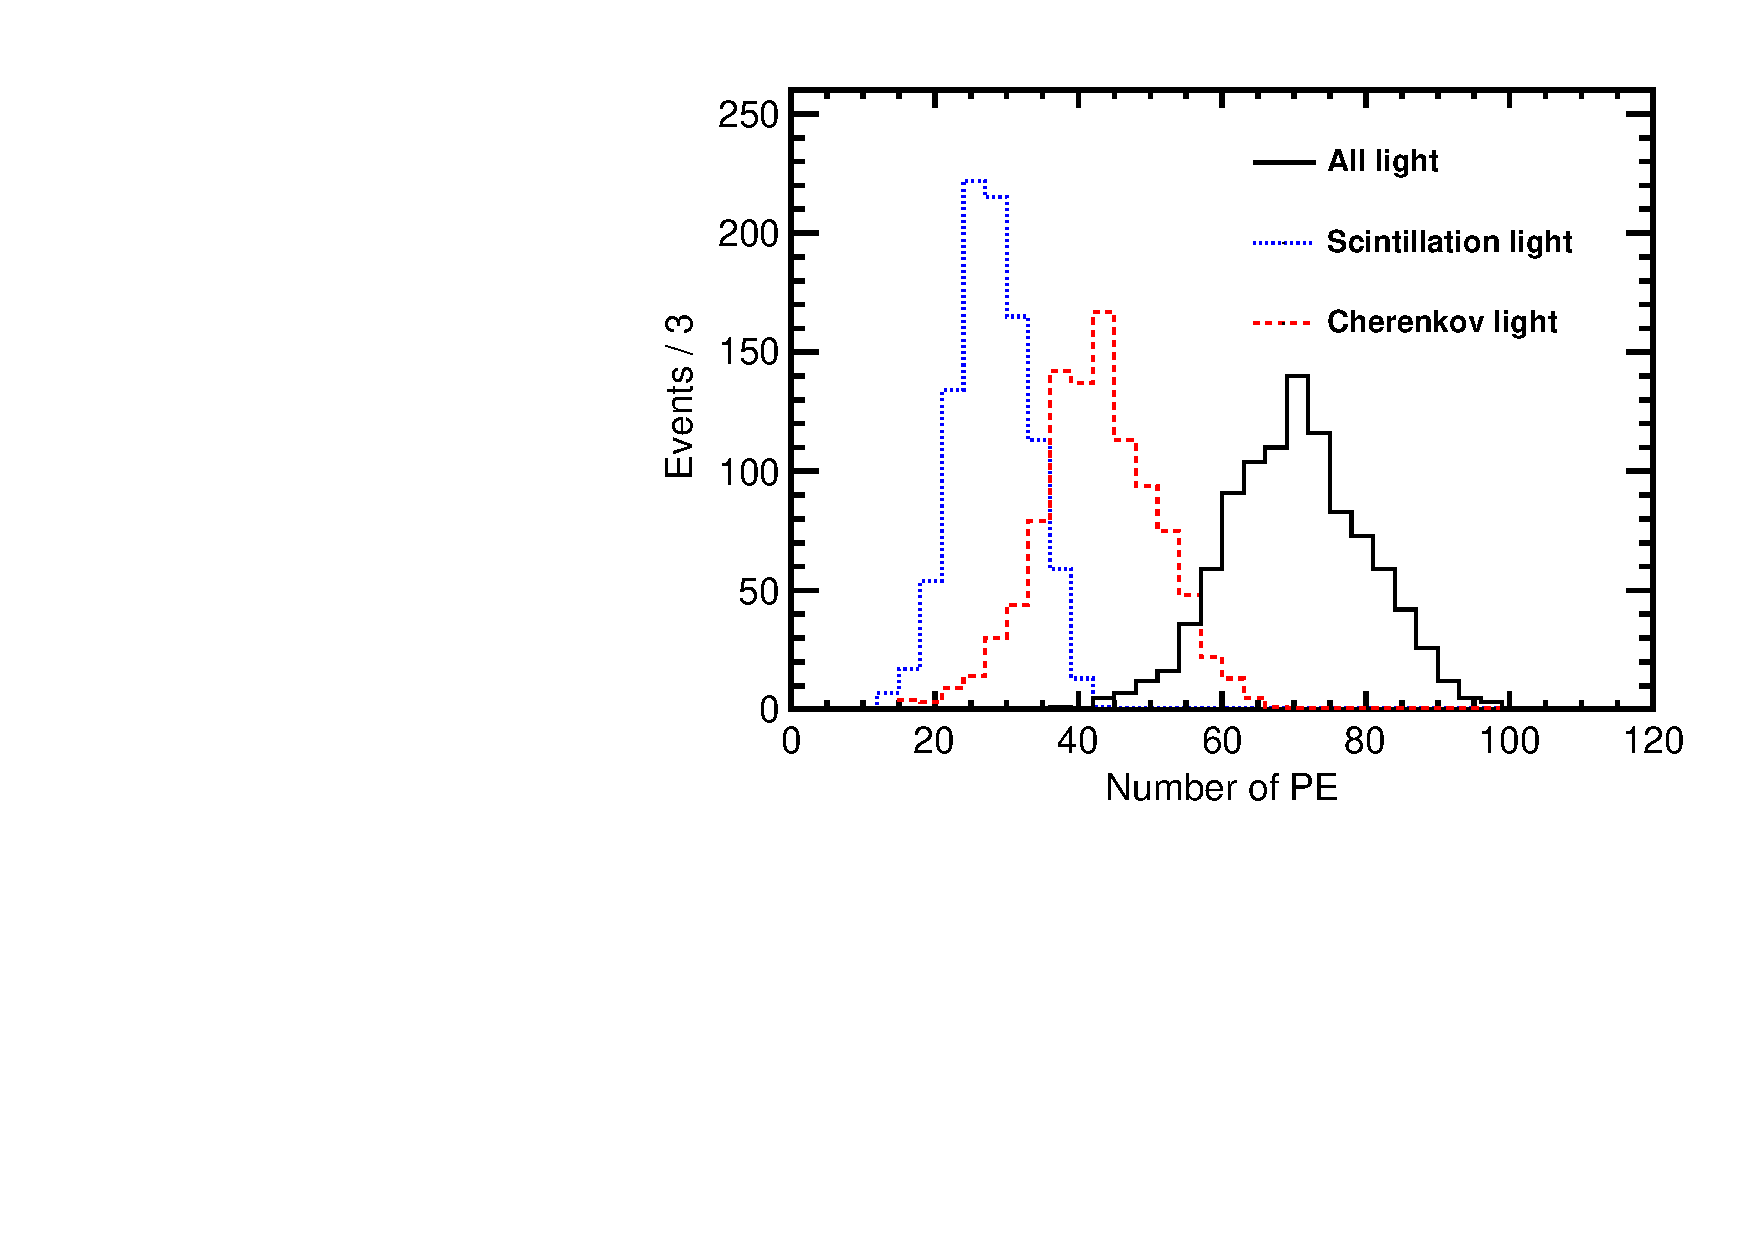
\includegraphics[width=0.45\textwidth]{hMomNPhot_1el_2p529MeV.pdf}
  \caption{Number of Cherenkov (\emph{dashed red line}), scintillation
    (\emph{dotted blue line}), and total (\emph{solid black line}) PEs
    for the simulation of 1000 $^{130}$Te 0{\nbb} decay (left panel)
    and $^8$B (\emph{right panel}) events.}
\label{fig:NPhotDist}
\end{figure*}

